%% LaTeX Beamer presentation template (requires beamer package)
%% see http://latex-beamer.sourceforge.net/
%% idea contributed by H. Turgut Uyar
%% template based on a template by Till Tantau
%% this template is still evolving - it might differ in future releases!

\PassOptionsToPackage{subsection=false}{beamerouterthememiniframes}
\documentclass{beamer}

\mode<presentation>
{
%\useoutertheme[subsection=false]{miniframes}
\usetheme{Berlin}
\setbeamertemplate{navigation symbols}{} 
\setbeamercovered{dynamic}
\setbeamertemplate{footline}{}
}

\hypersetup{pdfstartview={FitH}}

\usepackage[english]{babel}
\usepackage[utf8]{inputenc}
%\usepackage{lmodern}
\usepackage{mathptmx}% font definitions, try \usepackage{ae} instead of the following
\usepackage[scaled=.90]{helvet}% three lines if you don't like this look
\usepackage{courier}
\usepackage[T1]{fontenc}
\usepackage{url}
\usepackage{graphicx}
\usepackage{array}
\usepackage{colortbl}
\usepackage{tikz}
\usepackage{pgfplots}
\usepackage{colortbl}
\usepackage{xcolor}
\pgfplotsset{compat=1.7}

\definecolor{n_red}{HTML}{D7191C}
\definecolor{n_orange}{HTML}{FD9B61}
\definecolor{n_green}{HTML}{3F745A}
\definecolor{n_green_bg}{HTML}{AAE6C9}
\definecolor{n_blue}{HTML}{2B83BA}
\definecolor{n_violet}{HTML}{AC146D}
\definecolor{n_yellow}{HTML}{D2D221}
\definecolor{RawSienna}{cmyk}{0,0.72,1,0.45}
\definecolor{olive}{rgb}{0.3, 0.4, .1}

\newenvironment{colorblock}[3]{%
  \setbeamercolor{block body}{#2}
  \setbeamercolor{block title}{#3}
  \begin{block}{#1}}{\end{block}}
  
\title{A Survey on the Mathematical Emphasis in Brazilian Computer Science Curricula}

%\subtitle{}

% - Use the \inst{?} command only if the authors have different
%   affiliation.
%\author{F.~Author\inst{1} \and S.~Another\inst{2}}
\author[shortname]{Pedro Paulo Vezzá Campos \inst{1} \and \\
Jackson José Souza  \inst{1} \and \\
Giuliano Salcas Olguin \inst{2} \inst{3}}
\institute[shortinst]{
	\inst{1} Institute of Mathematics and Statistics --
		University of São Paulo, São Paulo, Brazil \\
	\{pedrovc, jackson\}@ime.usp.br \and
	\inst{2} Faculty of Education -- University of Campinas, Campinas, Brazil \and
	\inst{3} Polytechnic School -- University of São Paulo, São Paulo, Brazil \\
	giuliano.olguin@gmail.com}

\date{October 26, 2013}


% This is only inserted into the PDF information catalog. Can be left
% out.
\subject{A Survey on the Mathematical Emphasis in Brazilian Computer Science
Curricula}



% If you have a file called "university-logo-filename.xxx", where xxx
% is a graphic format that can be processed by latex or pdflatex,
% resp., then you can add a logo as follows:

% \pgfdeclareimage[height=0.5cm]{university-logo}{university-logo-filename}
% \logo{\pgfuseimage{university-logo}}



% Delete this, if you do not want the table of contents to pop up at
% the beginning of each subsection:
\AtBeginSection[]
{
\begin{frame}<beamer>
\frametitle{Contents}
\tableofcontents[currentsection,currentsubsection]
\end{frame}
}

% If you wish to uncover everything in a step-wise fashion, uncomment
% the following command:

%\beamerdefaultoverlayspecification{<+->}

\begin{document}

\begin{frame}
\titlepage
\end{frame}

\begin{frame}
\frametitle{Outline}
\begin{colorblock}{Introduction}{bg=n_violet!5}{bg=n_violet!100}
	\begin{itemize}
		\item Trends in higher education
		\item Decreasing focus in mathematics
	\end{itemize}
\end{colorblock}

\begin{colorblock}{Methodology \& Data}{bg=n_violet!5}{bg=n_violet!100}
	\begin{itemize}
		\item Mathematics in Brazilian CS programs
	\end{itemize}
\end{colorblock}

\begin{colorblock}{Conclusions}{bg=n_violet!5}{bg=n_violet!100}
	\begin{itemize}
		\item Is math actually loosing space?
	\end{itemize}
\end{colorblock}
%\tableofcontents
% You might wish to add the option [pausesections]
\end{frame}


%%%%%%%%%%%%%%%%%%%%%%%%%%%%%%%%%%%%%%%%%%%%%%%%%%%%%%%%%%%%%%%%%%%%%%%%%%%%%%%%
%%%%%%%%%%%%%%%%%%%%%%%%%%%%%%%%%%%%%%%%%%%%%%%%%%%%%%%%%%%%%%%%%%%%%%%%%%%%%%%%
\section{Introduction}
\subsection{}

%%%%%%%%%%%%%%%%%%%%%%%%%%%%%%%%%%%%%%%%%%%%%%%%%%%%%%%%%%%%%%%%%%%%%%%%%%%%%%%%
\begin{frame}
\frametitle{Trends in CS education}
\begin{columns}
\begin{column}{0.5\textwidth}
	\begin{colorblock}{Mission I}{bg=n_green_bg!30}{bg=n_green!100}
		\begin{itemize}
			\item Tackle current problems of society
			\item Focus on technical knowledge
		\end{itemize}
	\end{colorblock}
\end{column}
\begin{column}{0.5\textwidth}
	\begin{colorblock}{Mission II}{bg=n_green_bg!30}{bg=n_green!100}
		\begin{itemize}
			\item Glimpse the future
			\item Focus on academic knowledge
		\end{itemize}
	\end{colorblock}
\end{column}
\end{columns}

\end{frame}

%%%%%%%%%%%%%%%%%%%%%%%%%%%%%%%%%%%%%%%%%%%%%%%%%%%%%%%%%%%%%%%%%%%%%%%%%%%%%%%%
\begin{frame}
\frametitle{``Universities should educate -- employers should train''}

\begin{quote}
Universities are primarily in the business of positive human development. They
focus on enhancing the abilities of our graduates to
\textbf{\textcolor{n_red}{communicate clearly and effectively}}, to
\textbf{\textcolor{RawSienna}{analyze}}, to
\textbf{\textcolor{olive}{confront ambiguity}} with clear methods and
confidence, to \textbf{\textcolor{n_green}{break down problems}} into manageable parts, to
\textbf{\textcolor{n_blue}{think critically}}
and to \textbf{\textcolor{n_violet}{question deeply}}.\\
\hfill --- \textup{Max Blouw} \footnote{\tiny Blouw, M. (2013) ``Universities should
educate -- employers should train.'' [Online; accessed Oct 14, 2013] Available:
\url{http://www.theglobeandmail.com/commentary/universities-should-educate-employers-should-train/article14078938/}}
\end{quote}

\end{frame}

%%%%%%%%%%%%%%%%%%%%%%%%%%%%%%%%%%%%%%%%%%%%%%%%%%%%%%%%%%%%%%%%%%%%%%%%%%%%%%%%
\begin{frame}
\frametitle{The interplay between theory and practice}
The technology area is a strong example on how \textbf{\textcolor{olive}{standard procedures}} inside the
industry are \textbf{\textcolor{n_red}{constantly changing}}.

\begin{block}{Challenges}
	\begin{itemize}
		\item How can the university enable one to reason when facing new
		problems?
		\item How \emph{perennial}, fundamental should be the concepts taught?
		
	\end{itemize}
\end{block}

\end{frame}

%%%%%%%%%%%%%%%%%%%%%%%%%%%%%%%%%%%%%%%%%%%%%%%%%%%%%%%%%%%%%%%%%%%%%%%%%%%%%%%%
\begin{frame}
\frametitle{The interplay between theory and practice}
\begin{quote}
A fundamental aspect of computer science is the 
\textbf{\textcolor{n_red}{balance between theory and
practice and the essential link between them}}. Graduates of a computer science
program must understand not only the theoretical underpinnings of the discipline
but also how that \textbf{\textcolor{olive}{theory influences practice}}. \\
\hfill --- \textup{CS2008}
\footnote{\tiny ACM/IEEE Joint Task Force (2008) ``Computer Science Curriculum
2008: An interim revision of CS2001.''}

\end{quote}
\end{frame}

%%%%%%%%%%%%%%%%%%%%%%%%%%%%%%%%%%%%%%%%%%%%%%%%%%%%%%%%%%%%%%%%%%%%%%%%%%%%%%%%
\begin{frame}
\frametitle{Decreasing focus on mathematics}
\begin{itemize}
	\item CS is a \textbf{\textcolor{n_violet}{broad field}} that
	\textbf{\textcolor{n_blue}{connects to and draws from many disciplines}}, 
	including mathematics, electrical engineering, psychology, statistics, fine 
	arts, linguistics, and physical and life sciences.
	\item The \textbf{\textcolor{n_green}{role of mathematics}} in reference
	curricula has been \textbf{\textcolor{n_red}{decreasing gradually}} since at
	least the 1960s, although at a lower rate today. 
	\footnote{\tiny A. Ralston ``Do we need any mathematics in computer science
	curricula?'' \emph{SIGCSE Bull.}, vol 37, no. 2, pp 6-9, Jun 2005.}
	\footnote{\tiny A. B. Tucker ``Our curriculum has become math-phobic!'' in
	\emph{Proceedings of the Thirty-second SIGCSE Technical Symposium on
	Computer Science Education} ACM Press, 2001, pp. 243-247}

\end{itemize}

\end{frame}

%%%%%%%%%%%%%%%%%%%%%%%%%%%%%%%%%%%%%%%%%%%%%%%%%%%%%%%%%%%%%%%%%%%%%%%%%%%%%%%%
\begin{frame}
\frametitle{Case Study: Panorama on the study of mathematics in Brazil}
\begin{itemize}
	\item Overview of \textbf{\textcolor{n_red}{how much math}} is studied in
	eleven \textbf{\textcolor{n_blue}{well ranked Brazilian CS programs}}
	\item Objective analysis through a \textbf{\textcolor{n_violet}{quantitative analysis}}
	\item Comparison with reference curricula
	\item Useful for curriculum reforms
\end{itemize}
\end{frame}


%%%%%%%%%%%%%%%%%%%%%%%%%%%%%%%%%%%%%%%%%%%%%%%%%%%%%%%%%%%%%%%%%%%%%%%%%%%%%%%%
%%%%%%%%%%%%%%%%%%%%%%%%%%%%%%%%%%%%%%%%%%%%%%%%%%%%%%%%%%%%%%%%%%%%%%%%%%%%%%%%
\section{Methodology}
\subsection{}

%%%%%%%%%%%%%%%%%%%%%%%%%%%%%%%%%%%%%%%%%%%%%%%%%%%%%%%%%%%%%%%%%%%%%%%%%%%%%%%%
\begin{frame}
\frametitle{Definition of mathematics}
\begin{columns}
\begin{column}{0.5\textwidth}
	\begin{itemize}
		\item Calculus
		\item Linear Algebra
		\item Geometry
		\item Set Theory
	\end{itemize}
\end{column}
\begin{column}{0.5\textwidth}
	\begin{itemize}
		\item Algebra
		\item Discrete mathematics
		\item Probability
		\item Statistics
	\end{itemize}
\end{column}
\end{columns}

\end{frame}

%%%%%%%%%%%%%%%%%%%%%%%%%%%%%%%%%%%%%%%%%%%%%%%%%%%%%%%%%%%%%%%%%%%%%%%%%%%%%%%%
\begin{frame}
\frametitle{Selected CS Programs}
\begin{itemize}
	\item Brazil has more than \textbf{\textcolor{n_red}{350 CS programs}}
	\item The \textbf{\textcolor{n_green}{eleven}} selected ones were ranked as 
	\textbf{\textcolor{n_violet}{5-stars}} by the \emph{Guia do
	Estudante} ranking. 
	\item The ranking consists of an \textbf{\textcolor{olive}{opinion poll}} among professors, course
	coordinators and directors of departments.
	\item Each program is \textbf{\textcolor{RawSienna}{graded by six different reviewers}}, extremes are excluded
	\item Ranking audited by PricewaterhouseCoopers
\end{itemize}
\end{frame}

\section{Data}
\subsection{}

%%%%%%%%%%%%%%%%%%%%%%%%%%%%%%%%%%%%%%%%%%%%%%%%%%%%%%%%%%%%%%%%%%%%%%%%%%%%%%%%
\begin{frame}
%\frametitle{Map of Brazil}
\begin{figure}[htp]
\begin{center}
  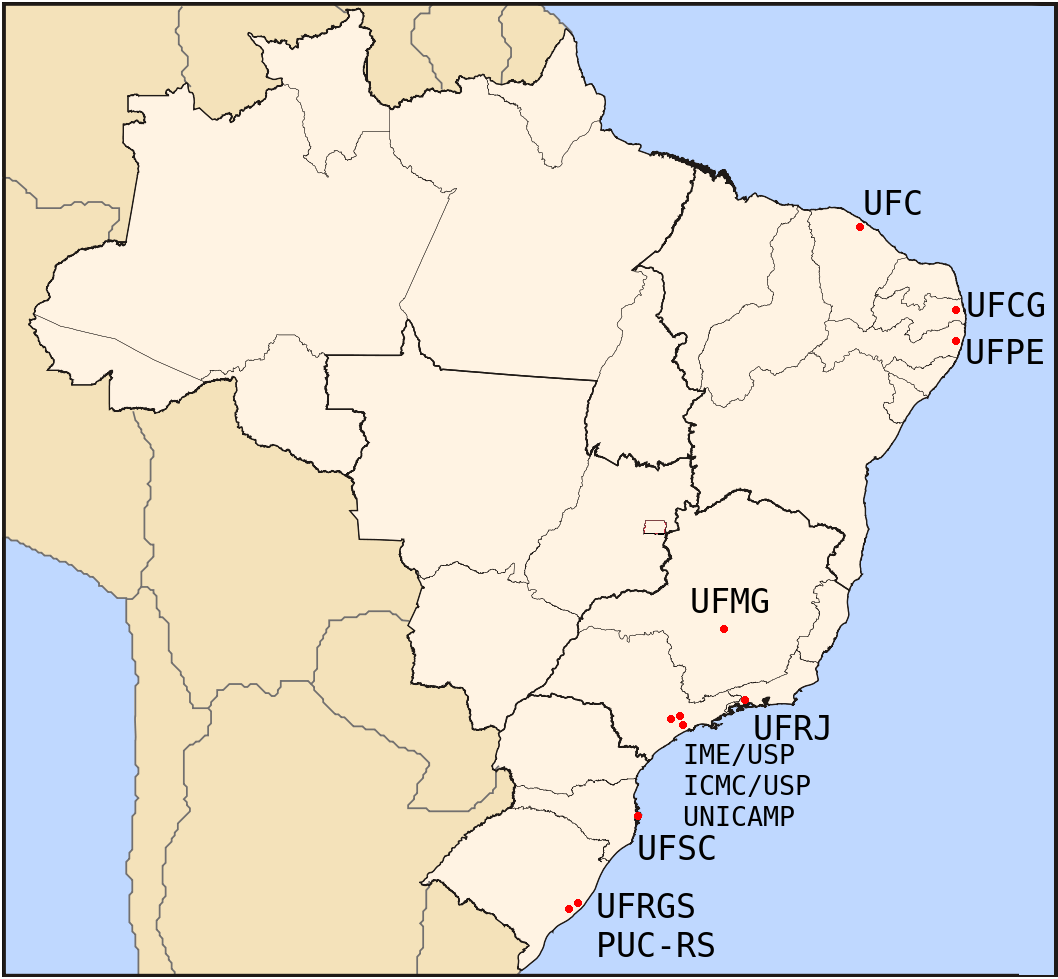
\includegraphics[height=7cm]{brazil_map.png}
  \caption[map]{Map of Brazil with the studied universities \footnote{\tiny
  Image courtesy of Wikipedia, the Free Encyclopedia}}
\end{center}
\end{figure}

\end{frame}

%%%%%%%%%%%%%%%%%%%%%%%%%%%%%%%%%%%%%%%%%%%%%%%%%%%%%%%%%%%%%%%%%%%%%%%%%%%%%%%%
\begin{frame}
\begin{table}
	\scriptsize
	\caption{Studied CS Programs Panorama}
    \begin{tabular}{|c|c|c|c|c|c|c|}
        \hline
        University  & Period    & Organization & Foundation   \\ \hline
        \rowcolor[gray]{.8}
        ICMC/USP    & Diurnal   & Public       & 1979         \\ 
        \rowcolor[gray]{.8}
        IME/USP     & Diurnal   & Public       & 1970         \\ 
        PUC-RS      & Nocturnal & Private      & 1983         \\ 
        UFC         & Diurnal   & Public       & 1975         \\ 
        UFCG        & Diurnal   & Public       & 1977         \\ 
        UFMG        & Diurnal   & Public       & 1978         \\ 
        UFPE        & Diurnal   & Public       & 1974         \\ 
        UFRGS       & Diurnal   & Public       & 1983         \\ 
        \rowcolor[gray]{.8}
        UFRJ        & Diurnal   & Public       & 1974         \\ 
        UFSC        & Diurnal   & Public       & 1976         \\ 
        UNICAMP     & Nocturnal & Public       & 1969         \\
        \hline
    \end{tabular}
\end{table}
\end{frame}

%%%%%%%%%%%%%%%%%%%%%%%%%%%%%%%%%%%%%%%%%%%%%%%%%%%%%%%%%%%%%%%%%%%%%%%%%%%%%%%%
\begin{frame}
\begin{table}
	\scriptsize
	\caption{Studied CS Programs Panorama}
    \begin{tabular}{|c|c|c|c|c|c|c|}
        \hline
        University   & Years & Students/year & Where is located                                   \\ \hline
        \rowcolor[gray]{.8}
        ICMC/USP     & 5     & 100   & Institute of Mathematical Sciences and CS        \\ 
        \rowcolor[gray]{.8}
        IME/USP      & 4     & 50    & Institute of Mathematics and Statistics          \\ 
        PUC-RS       & 4     & 60    & Faculty of Informatics                           \\ 
        UFC          & 4     & 60    & Center of Sciences                               \\ 
        UFCG         & 4     & 90    & Center of Eletrical Engineering and Informatics  \\ 
        UFMG         & 4     & 80    & Institute of Exact Sciences                      \\ 
        UFPE         & 4.5   & 100   & Center of Informatics                            \\ 
        UFRGS        & 4.5   & 100   & Institute of Informatics                         \\ 
        \rowcolor[gray]{.8}
        UFRJ         & 4.5   & 50    & Institute of Mathematics                         \\ 
        UFSC         & 4     & 100   & Institute of Informatics and Statistics          \\ 
        UNICAMP      & 5     & 50    & Institute of Computing                           \\
        \hline
    \end{tabular}
\end{table}
\end{frame}

%%%%%%%%%%%%%%%%%%%%%%%%%%%%%%%%%%%%%%%%%%%%%%%%%%%%%%%%%%%%%%%%%%%%%%%%%%%%%%%%
\begin{frame}
\begin{figure}[!t]
\centering
\includegraphics{../chart_math_two_colors.pdf}
\caption{The proportion of mathematics in each curriculum compared with the reference curricula}
\label{chart_math}
\end{figure}

\end{frame}


%%%%%%%%%%%%%%%%%%%%%%%%%%%%%%%%%%%%%%%%%%%%%%%%%%%%%%%%%%%%%%%%%%%%%%%%%%%%%%%%
%%%%%%%%%%%%%%%%%%%%%%%%%%%%%%%%%%%%%%%%%%%%%%%%%%%%%%%%%%%%%%%%%%%%%%%%%%%%%%%%
\section{Conclusions}
\subsection{}

%%%%%%%%%%%%%%%%%%%%%%%%%%%%%%%%%%%%%%%%%%%%%%%%%%%%%%%%%%%%%%%%%%%%%%%%%%%%%%%%
\begin{frame}
\frametitle{Future work}
\begin{itemize}
	\item Reapply the analysis with \textbf{\textcolor{n_red}{other rankings}}
	(Eg. ENADE ranking made by the Brazilian Ministry of Education)
	\item Is there any \textbf{\textcolor{olive}{correlation}} between being
	\textbf{\textcolor{n_violet}{well ranked}} and the
	\textbf{\textcolor{RawSienna}{amount of math}} studied?
	\item How \textbf{\textcolor{n_green}{useful}} was mathematics after
	graduation? Apply \textbf{\textcolor{n_blue}{questionnaires}} to
	analyze the strengths and weaknesses of
	a curriculum.
\end{itemize}
\end{frame}

%%%%%%%%%%%%%%%%%%%%%%%%%%%%%%%%%%%%%%%%%%%%%%%%%%%%%%%%%%%%%%%%%%%%%%%%%%%%%%%%
\begin{frame}
\frametitle{This paper}
\begin{itemize}
	\item Analyzed the \textbf{\textcolor{n_red}{different perspectives}} of
	teaching at universities and \textbf{\textcolor{n_green}{opinions}} related
	\item Noted the \textbf{\textcolor{n_violet}{decline}} of the teaching of
	\textbf{\textcolor{RawSienna}{mathematics}} in CS both as a trend in reference
	curricula and in eleven
	different CS programs in Brazil
\end{itemize}
\end{frame}

%%%%%%%%%%%%%%%%%%%%%%%%%%%%%%%%%%%%%%%%%%%%%%%%%%%%%%%%%%%%%%%%%%%%%%%%%%%%%%%%
\begin{frame}
\frametitle{}

\begin{center}
\Huge Thanks! \\
\Large Questions?
\end{center}

\end{frame}









%\begin{frame}
%\begin{table}
%	\centering
%	\caption{math coverage in Brazilian CS curricula}
%    \begin{tabular}{|c|>{\centering\arraybackslash}m{1cm}|>{\centering\arraybackslash}m{1cm}|>{\centering\arraybackslash}m{2cm}|}
%        \hline
%        University   & Total math hours & Total curricular hours & Percentage of math in curriculum \\ \hline
%		\rowcolor[gray]{.9}
%        ACM/IEEE     & 39   & 280        & 13.93\%                          \\ 
%		\rowcolor[gray]{.9}
%        SBC (4 years)& 30   & 160        & 18.75\%                          \\ 
%        ICMC/USP     & 540  & 4395       & 12.29\%                          \\ 
%        IME/USP      & 750  & 2985       & 25.13\%                          \\ 
%        PUC-RS       & 300  & 3045       & 9.85\%                           \\ 
%        UFC          & 400  & 3280       & 12.20\%                          \\ 
%        UFCG         & 420  & 3120       & 13.46\%                          \\ 
%        UFMG         & 540  & 2625       & 20.57\%                          \\ 
%        UFPE         & 285  & 3495       & 8.15\%                           \\ 
%        UFRGS        & 360  & 3240       & 11.11\%                          \\ 
%        UFRJ         & 480  & 3075       & 15.61\%                          \\ 
%        UFSC         & 486  & 3528       & 13.78\%                          \\ 
%        UNICAMP      & 510  & 3000       & 17.00\%                          \\
%        \hline
%    \end{tabular}
%\end{table}
%\end{frame}


%\begin{frame}
%\frametitle{Bibliografia}
%{\small
%	\bibliographystyle{alpha}% citação bibliográfica alpha
%	\bibliography{../bibliography}  % associado ao arquivo: 'bibliografia.bib'
%}
%\end{frame}

\end{document}

